\part{Conception}

\chapter{Conception générale}

\section{Répartition en paquetage}

Dans notre projet, nous avons un paquetage par défaut \textit{stockgestion}. Dans ce paquetage, nous retrouvons 5 sous-paquetages \textit{Entite}, \textit{Manager}, \textit{Controlleur}, \textit{Outil} et \textit{UI}.\\

Chaque package a des fonctionnalitées bien délimité. 
\begin{itemize}
	\item UI regroupe toutes les classes de l'interface utilisateur.
	\item Manager s'occupe de toutes les intéractions avec la base de donnée.
	\item Controlleur gèrent les interactions entre toutes les classes et les actions de l'utilisateur.
	\item Outil contient toutes les classes Outils
	\item Entite contient toutes les représentations objets de notre application.
\end{itemize}

Ci-dessous, le diagramme de Package qui représente les interactions entre nos packages :
\begin{center}
	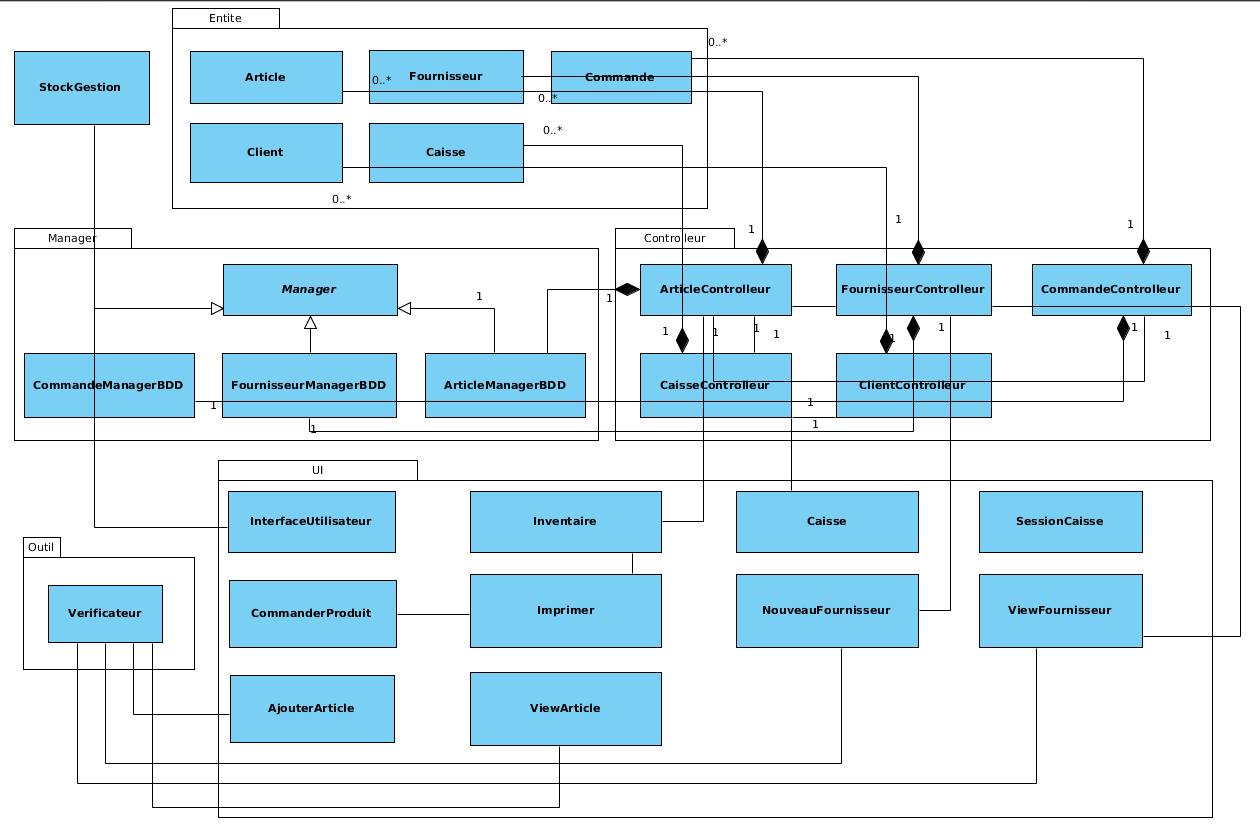
\includegraphics[width=14cm]{Conception/DiagrammeDeClassePackage.png}
\end{center}

\begin{center}
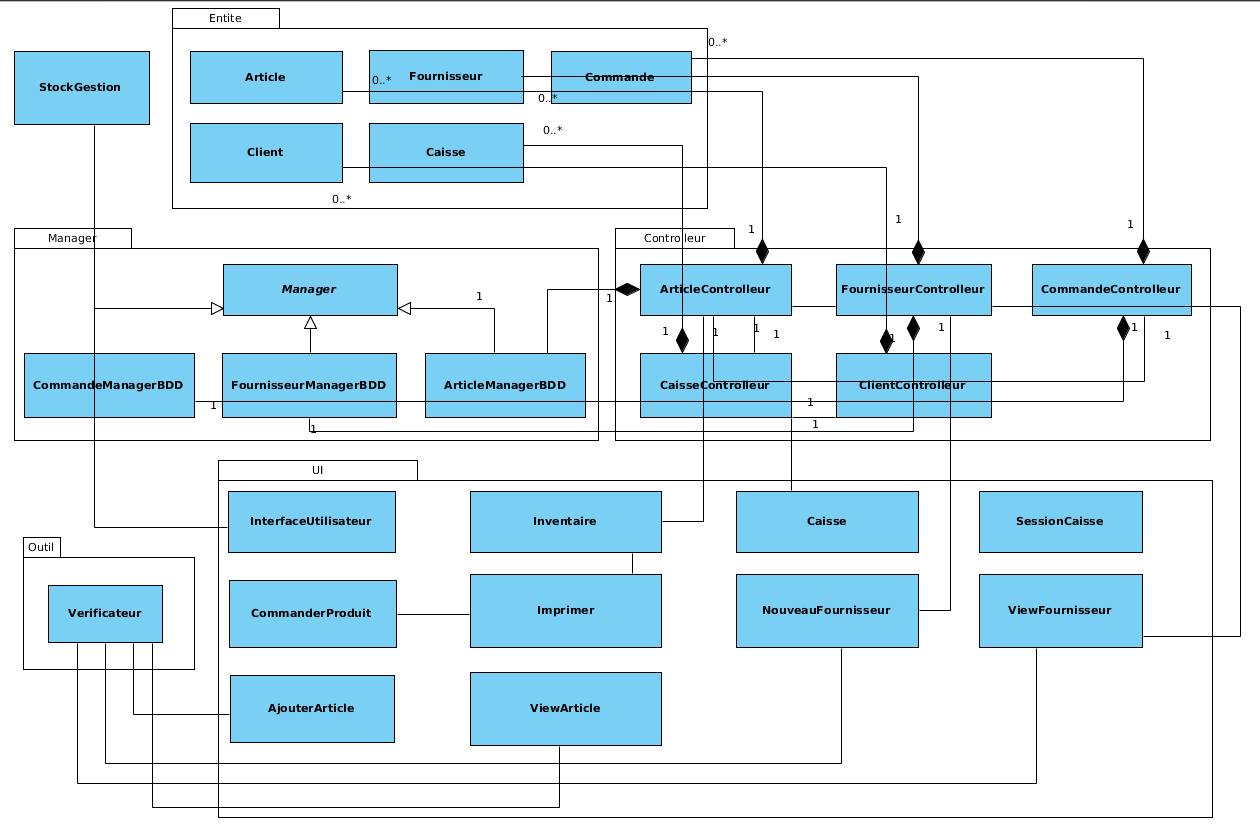
\includegraphics[width=14cm]{./Conception/DiagrammeDeClassePackage}
\end{center}

\section{Choix des technologies}
Le projet consiste à implémenter une solution de suivi de stock et de gestion d'une caisse. Elle ne requiert aucun traitement lourd, nous n'avons donc pas implémenter de traitement multithread. 

Notre projet est bâti autour d'un MVC comprenant un package de controlleurs, un package de vue et un package de manager. Les managers traitent avec une base de donnée SQL nommé Derby. Nous avons fait ce choix car ils nous semblait important de stocker les données dans une base de donnée type SQL. De plus, nous avions déjà travailler avec Derby dans des projets précédents.

L'interface utilisateur est animé par swing. Ce fût un choix pratique avant tous, notamment car Neteans propose un générateur de template puissant nommé Matisse.

Notre solution compte également de nombreux Singleton. En effet, les controlleurs et les managers sont des singletons. La raison de cette implémentation a déjà été expliqué dans la aprtie précédente.

\section{Diagramme de composant du logiciel}

Quentin ?

\section{Diagramme de déploiement}

Ngocky ?


\chapter{Conception détaillée}

\section{Diagrammes de classes techniques des paquetages}

A la racine de notre projet, nous retrouvons le paquetage \textbf{stockgestion} créé par défaut. Ce paquetage ne contient qu'une seule classe \textbf{StockGestion} qui a le rôle d'initialiser et de rafraîchir toutes les interfaces d'utilisateur lors des changements dans les données.

\begin{center}
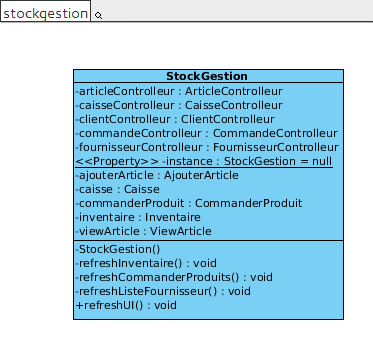
\includegraphics[width=14cm]{./Conception/stockgestion}
\end{center}

Dans le paquetage \textbf{stockgestion}, nous retrouvons 5 sous-paquetages. Chacun contient des classes qui jouent un certain rôle précis dans l'application.\\

Premièrement, nous avons le paquetage \textbf{Entite}. Dans ce paquetage, chaque classe représente une entité utilisé dans l'application: un article, un fournisseur, une commande, un client ou encore une caisse.

\begin{center}
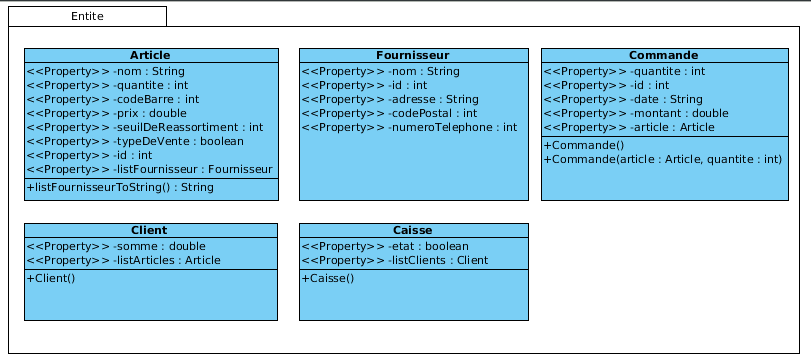
\includegraphics[width=14cm]{./Conception/entite}
\end{center}

Ensuite, nous avons le paquetage \textbf{Manager}. Chaque classe dans ce paquetage s'occupe de la connexions avec la base de données ainsi que de toutes les opérations liées à cette base.\\
Nous retrouvons ici la classe mère \textbf{Manager} qui contient la méthode de connexion à Derby. Nous avons 3 classes filles, chacune s'occupe des opération des articles, des commandes et des fournisseurs respectivement.

\begin{center}
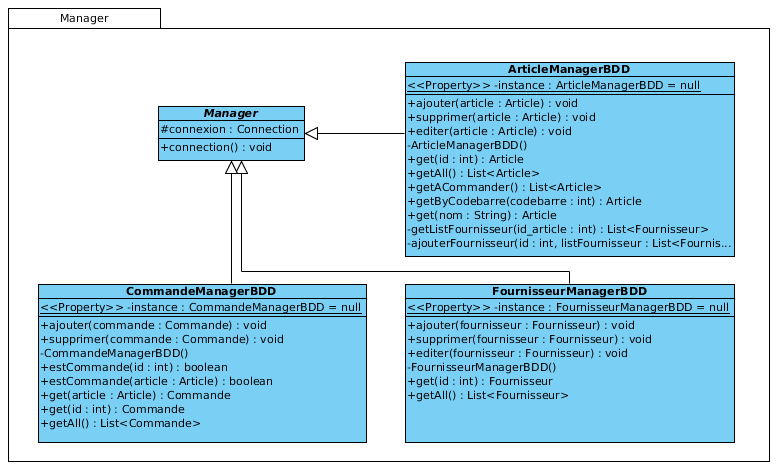
\includegraphics[width=14cm]{./Conception/manager}
\end{center}

Nous avons le paquetage \textbf{Controleur} qui contient des classes de contrôleurs. Ces classes réalisent les opérations sur les entités en appelant les méthodes des managers.

\begin{center}
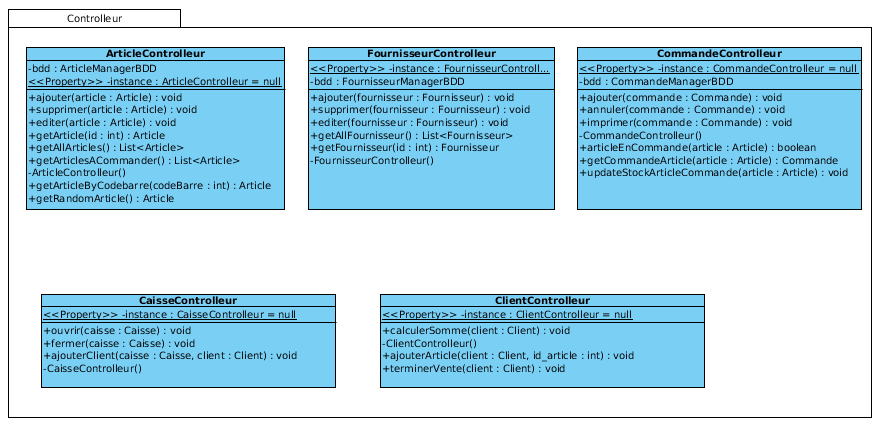
\includegraphics[width=14cm]{./Conception/controlleur}
\end{center}

Pour les besoins très spécifiques de notre application, nous avons créé le paquetage \textbf{Outil}. On y trouve la classe \textbf{Verificateur} qui s'occupe de toutes les vérifications des entrées utilisateurs de notre application, ainsi permet d'éviter des erreurs avec la base de données (un numéro mal écrit, un texte avec des caractères spéciaux...).

\begin{center}
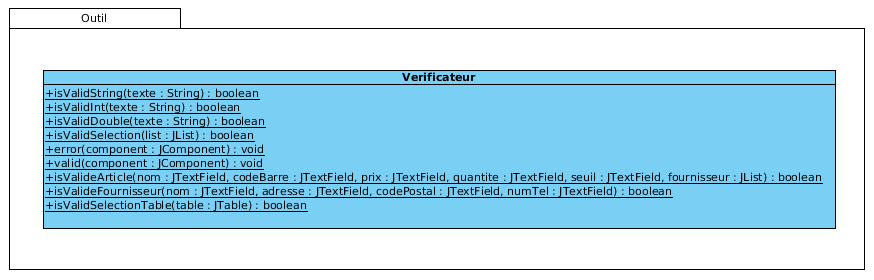
\includegraphics[width=14cm]{./Conception/outil}
\end{center}

Enfin, nous avons le paquetage \textbf{UI} qui contient toutes les classes de notre interface utilisateur. Chaque classe représente une fenêtre différente, chaque fenêtre correspond à une fonctionnalité de notre application.

\begin{center}
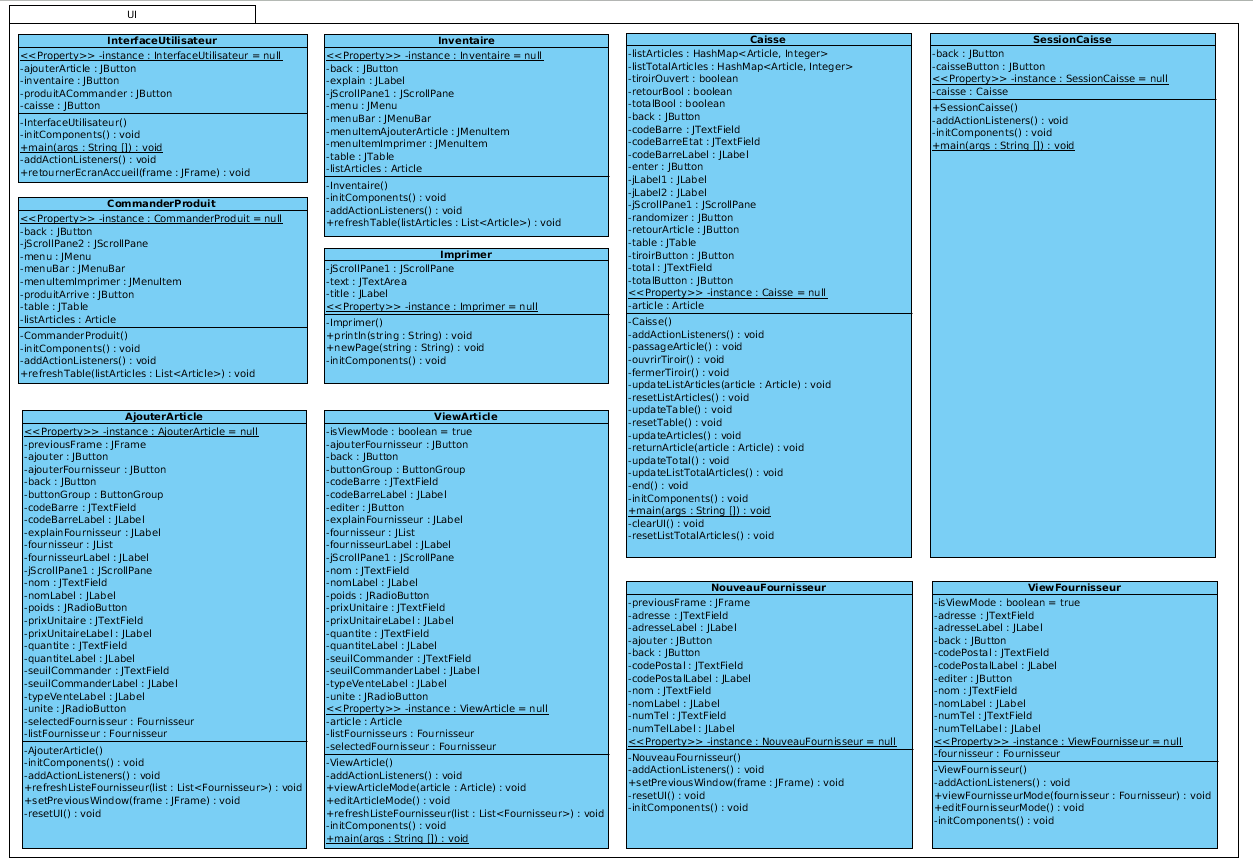
\includegraphics[width=14cm]{./Conception/ui}
\end{center}


\section{Diagrammes de séquences techniques}

Quentin ?

\section{Architecture du projet: approche MVC}
Notre application repose sur une architecture MVC. Les vues, les controllers et les managers sont ainsi séparés et placés dans des packages différents.
Comme illustré plusieurs fois, le package UI s'occupe de l'aspect vue du modèle MVC.
Le package Manager correspondant au manager et s'occupe de toutes les transactions avec la base de donnée.

Enfin le package controlleur contient tous les contrôleurs et gèrent toutes les actions de l'utilisateur. 